\documentclass[a4paper, 12pt, final, garamond]{book}
\usepackage{cours-preambule}

\raggedbottom

\makeatletter
\renewcommand{\@chapapp}{M\'ecanique -- chapitre}
\makeatother

\begin{document}
\setcounter{chapter}{2}

\chapter{TD entra\^inement~: mouvements courbes}
\section{Glissade d'un pingouin sur un igloo}

\hspace*{-0.75cm}
\begin{minipage}{0.70\linewidth}
    Un pingouin, assimilable à un point matériel M de masse $m$ décide de faire
    du toboggan. Il s'élance sans vitesse initiale du sommet A d'un igloo
    voisin, assimilable à une demi sphère $S$ de rayon $R$ et de centre O, posée
    sur un plan horizontal $\Pi$. On considère que le glissement s'effectue sans
    frottement dans le plan vertical ($x$O$z$).
\end{minipage}
\hfill
\begin{minipage}{0.25\linewidth}
    \begin{center}
        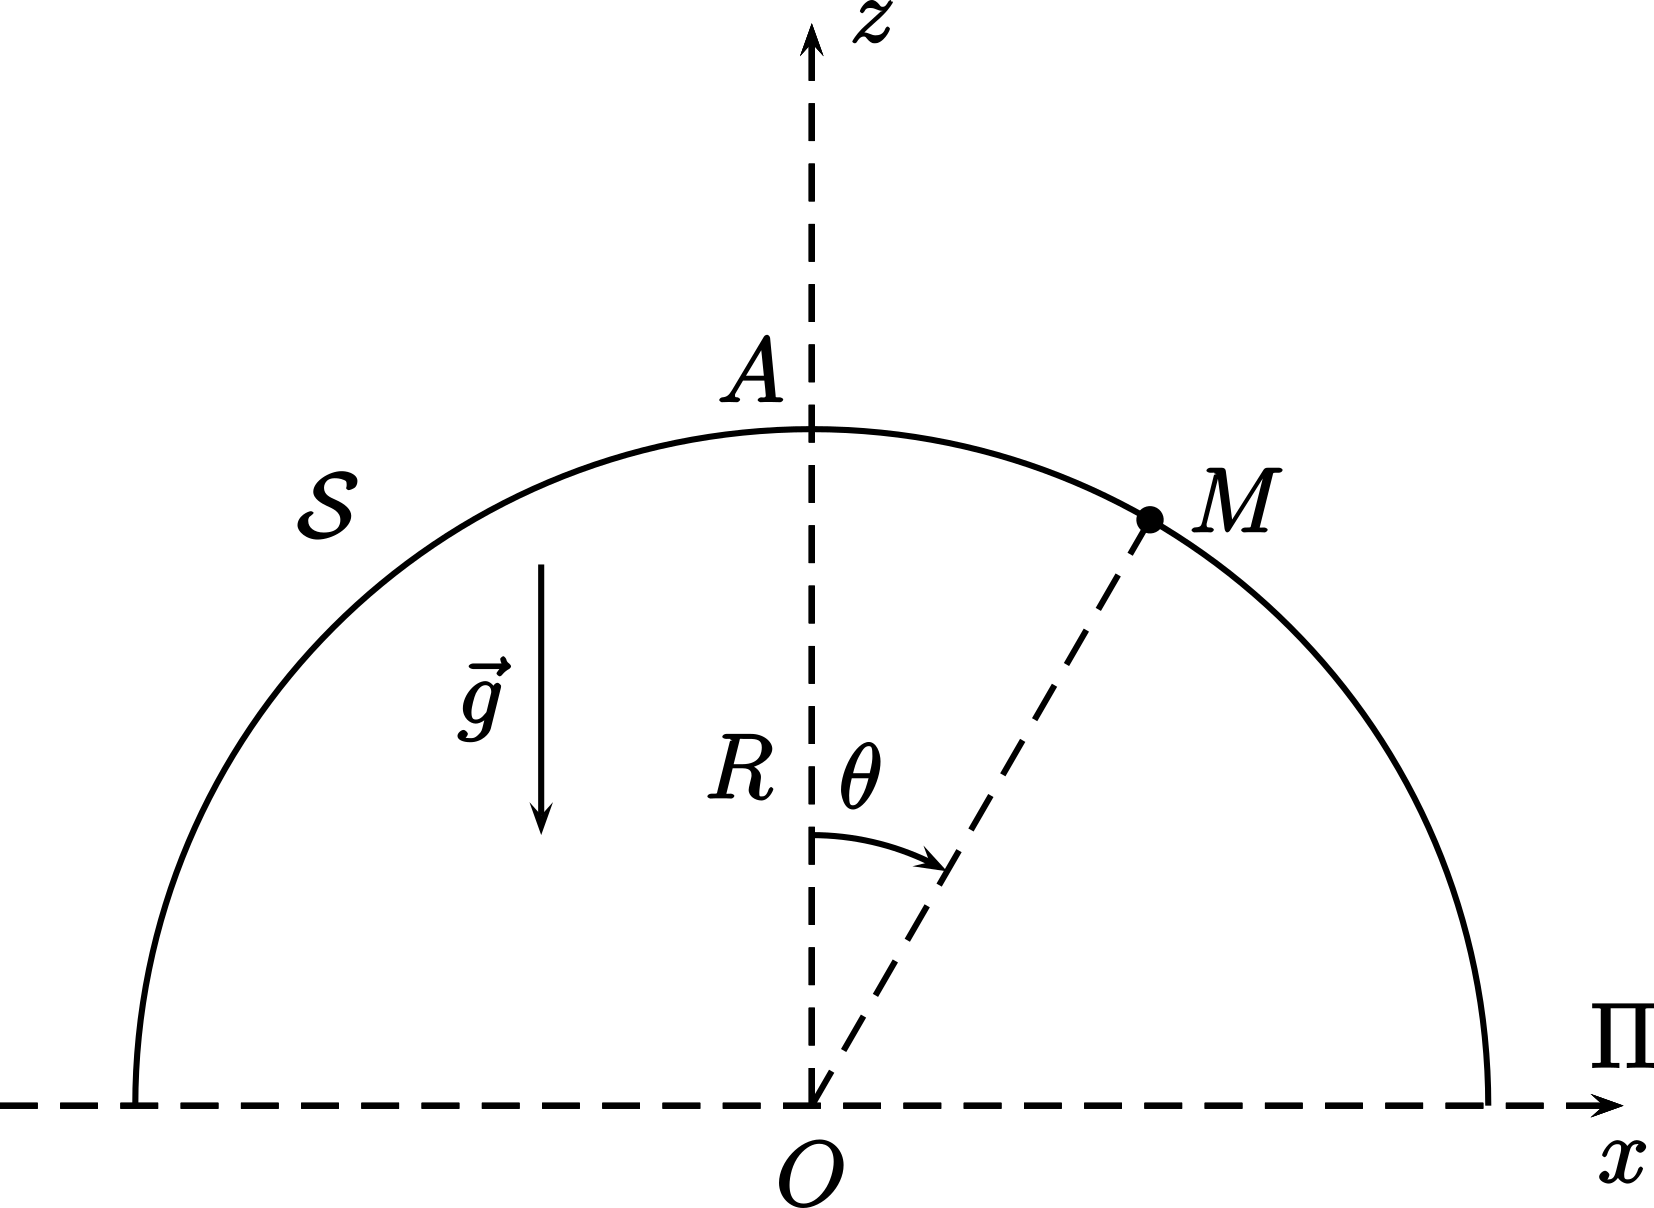
\includegraphics[width=\linewidth]{igloo-plain}
    \end{center}
\end{minipage}

\begin{enumerate}
    \item Appliquer le PFD au pingouin pour en déduire deux équations
        différentielles portant sur l'angle $\tt$. Identifier l'équation du
        mouvement qui permet de déterminer $\tt(t)$. Quelle information l'autre
        information contient-elle~?
    \item En multipliant l'équation du mouvement par $\tp$ et en intégrant sur
        $t$, montrer que
        \[\tp^2 = \frac{2g}{R}(1-\cos\tt)\]
    \item En déduire la norme de la force de réaction de l'igloo.
    \item Le pingouin décolle-t-il du toit de l'igloo avant d'atteindre le sol~?
        Si oui, pour quel angle~?
\end{enumerate}

\section{Course de F1}
\hspace*{-0.75cm}
\begin{minipage}{0.70\linewidth}
    Lors des essais chronométrés d'un grand prix, Fernando \textsc{Alonso} (point A)
    et Jenson \textsc{Button} (point B) arrivent en ligne droite et coupent l'axe
    $\D$ au même instant de leur parcours. Ils prennent cependant le virage de deux
    façons différentes~: \bigbreak
    \begin{itemize}
        \item \textsc{Alonso} suit une trajectoire circulaire de rayon $R_A =
            \SI{90.0}{m}$~;
        \item \textsc{Button} choisit une trajectoire de rayon $R_B = \SI{75.0}{m}$.
    \end{itemize} \bigbreak
    On cherche à déterminer quelle est la meilleure trajectoire, c'est-à-dire
    lequel des deux pilote gagne du temps par rapport à l'autre à la sortie du
    virage.
\end{minipage}
\hfill
\begin{minipage}{0.25\linewidth}
    \begin{center}
        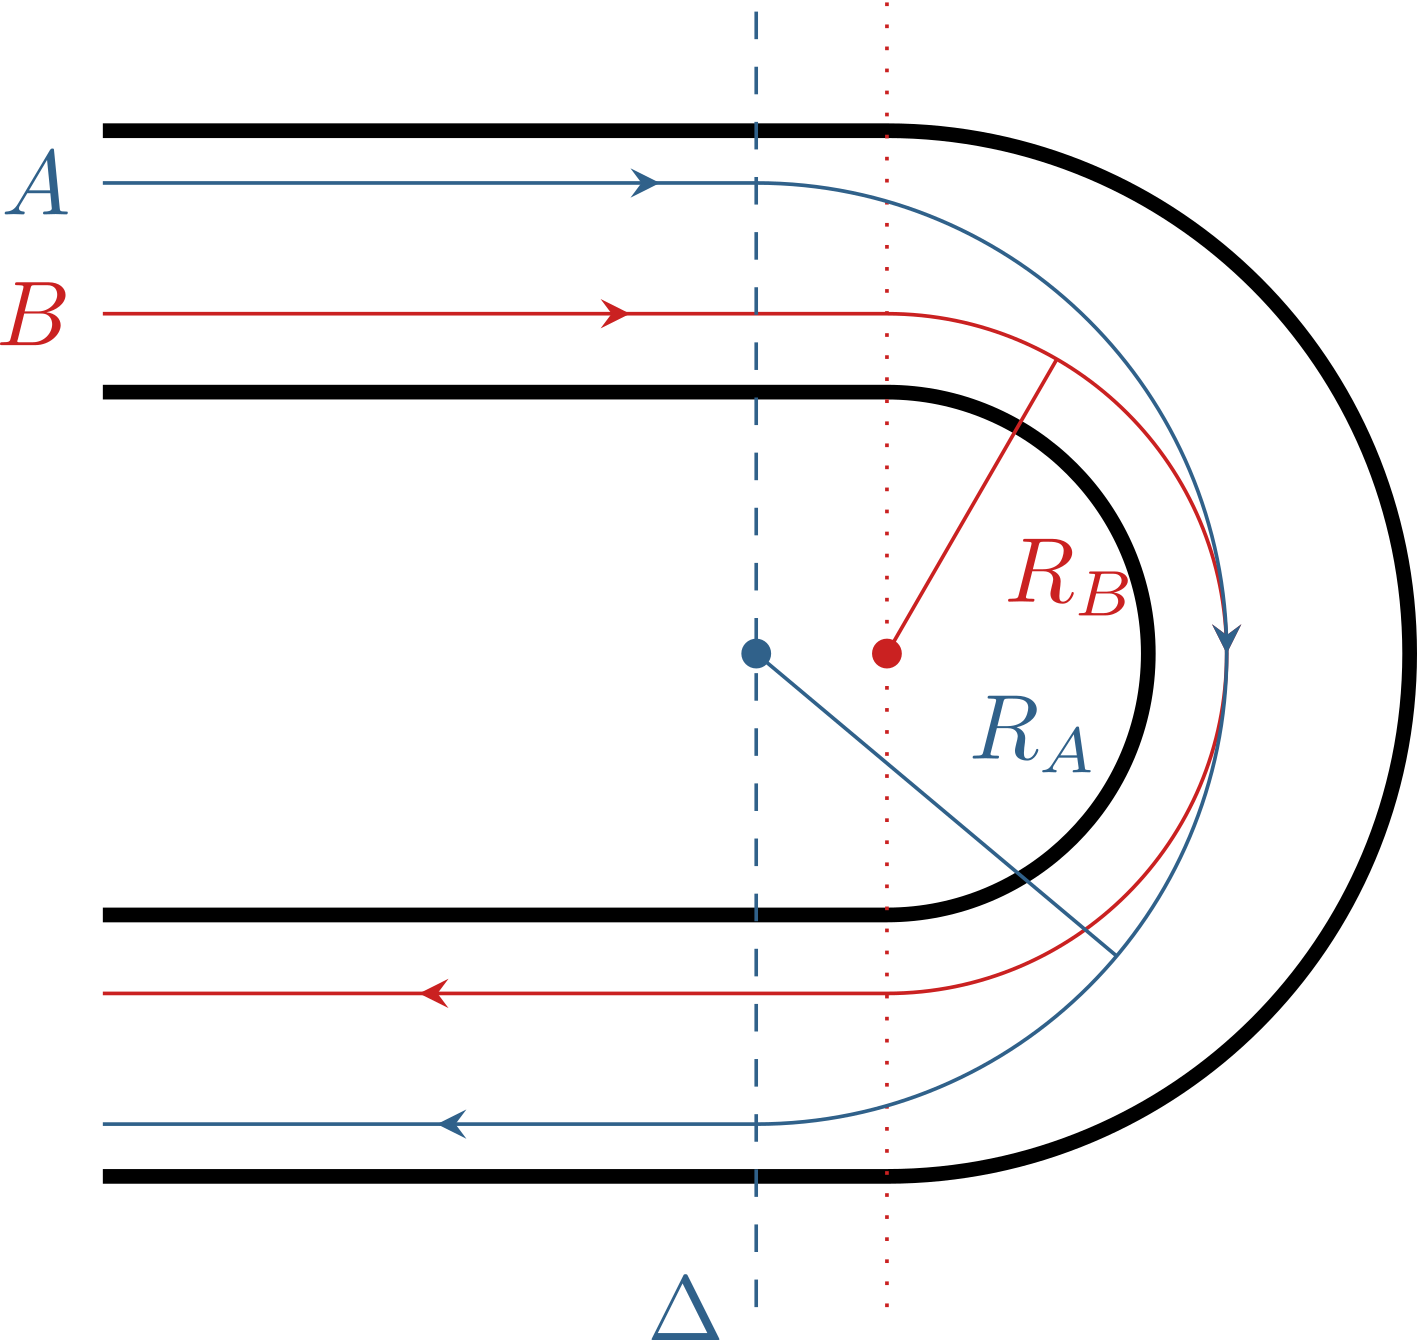
\includegraphics[width=\linewidth]{F1_plain}
    \end{center}
\end{minipage}
\bigbreak
\begin{enumerate}
    \item Déterminer les distances $D_A$ et $D_B$ parcourues par les deux
        pilotes entre leurs deux passages par l'axe $\D$. Que peut-on conclure~?
    \item Pour simplifier, on imagine que les deux voitures roulent à des
        vitesse $v_A$ et $v_B$ constantes entre leurs deux passages par l'axe
        $\D$. Déterminer ces vitesses, sachant que l'accélération des voitures
        doit rester inférieur à \SI{0.8}{g} sous risque de dérapage. Les
        calculer numériquement.
    \item Conclure quant à la meilleure trajectoire des deux.
\end{enumerate}

%\vspace*{-20pt}
\section{Entraînement d'une spationaute}

\hspace*{-0.75cm}
\begin{minipage}{0.70\linewidth}
    Une spationaute doit subir différents tests d'aptitude aux vols spatiaux,
    notamment le test des accélérations. Pour cela, on l'installe dans une
    capsule de centre S, fixée au bout d'un bras métallique horizontal dont
    l'autre extrémité est rigidement liée à un arbre de rotation vertical $\D$.
    La longueur du bras est notée $L$. On assimilera la spationaute au point
    matériel S. \bigbreak
\end{minipage}
\hfill
\begin{minipage}{0.25\linewidth}
    \begin{center}
        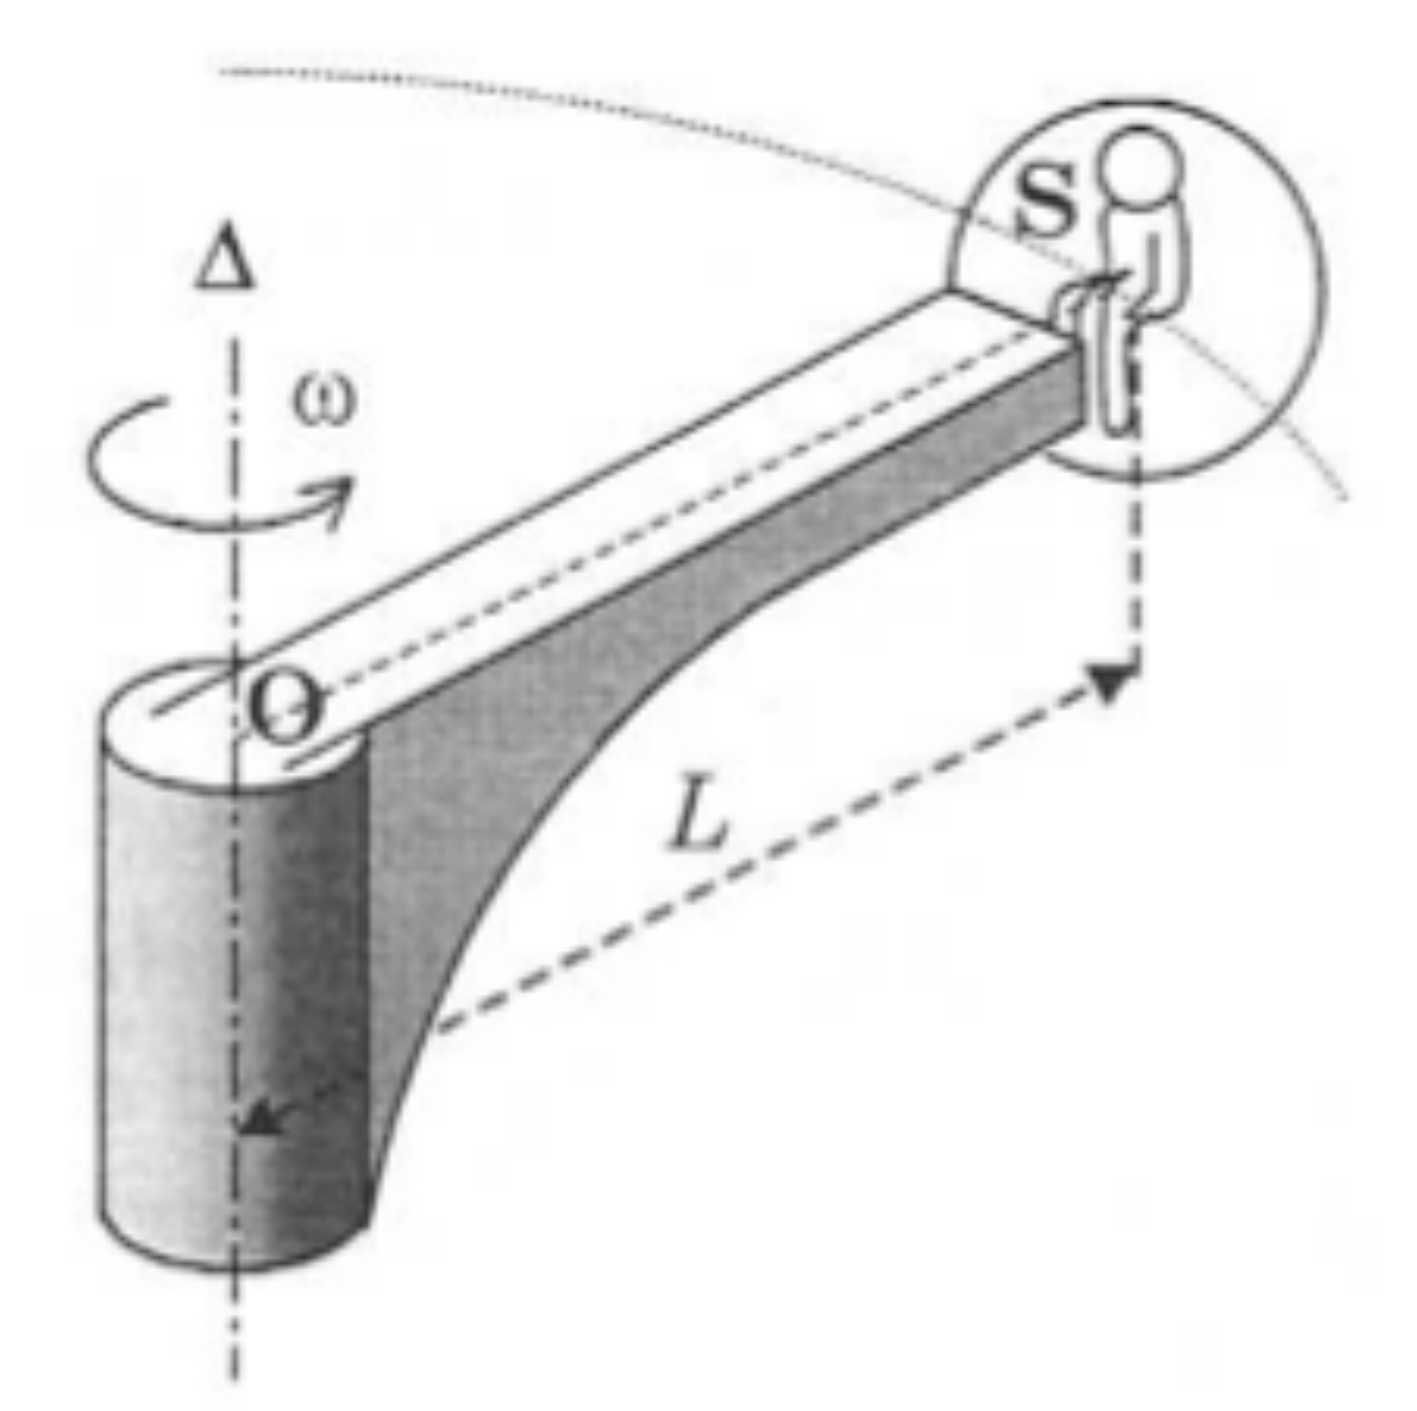
\includegraphics[width=\linewidth]{centri_spat-plain}
    \end{center}
\end{minipage}

L'ensemble \{capsule + bras + arbre\} est mis en rotation avec un vitesse
angulaire croissant progressivement selon la loi
\[\w(t) = \w_0(1-\exp^{-t/\tau})\]
avec $\w_0$ la vitesse angulaire nominale du simulateur, et $\tau$ un temps
caractéristique. On donne $L = \SI{10.0}{m}$ et $g = \SI{9.81}{m.s^{-2}}$.
\bigbreak
\begin{enumerate}
    \item Dessiner la trajectoire de la spationaute ainsi que son vecteur
        vitesse dans le référentiel du laboratoire, en faisant figure la base
        adaptée à l'étude de ce mouvement.
    \item Donner l'expression des vecteurs position, vitesse et accélération de
        la spationaute à un instant $t$ quelconque dans le référentiel du
        laboratoire.
    \item À partir de quelle durée peut-on supposer que le mouvement est
        circulaire et uniforme~? Que deviennent les expressions des vecteurs
        vitesse et accélération dans ce cas~? Calculer alors la norme de
        l'accélération subie par la spationaute.
    \item Quelle doit être la valeur de $\w_0$ pour que l'accélération atteigne
        \SI{10}{g} lors du régime de rotation uniforme~? On donnera le résultat
        en tours par second.
\end{enumerate}

\section{Anneau sur une tige en rotation}

\hspace*{-0.75cm}
\begin{minipage}{0.70\linewidth}
    On considère un petit anneau M de masse $m$ considéré comme ponctuel, soumis
    à la pesanteur et susceptible de se déplacer sans frottement le long d'une
    tige OA horizontale dans le plan ($x$O$y$), de longueur $\ell$, effectuant
    des mouvements de rotation caractérisés par une vitesse angulaire $\w$
    constante autour d'un axe fixe vertical $\D$ passant par son extrémité O. Le
    référentiel lié au laboratoire est considéré comme galiléen. On considère~:
    \bigbreak
    \begin{itemize}
        \item le repère cartésien $(\Or,\ex,\ey,\ez)$ fixe dans le référentiel
            du laboratoire et associé aux axes $x$, $y$ et $z$~;
        \item la base cylindrique locale $(\er,\et,\ez)$ associée au point M.
    \end{itemize}
    \bigbreak
\end{minipage}
\hfill
\begin{minipage}{0.25\linewidth}
    \begin{center}
        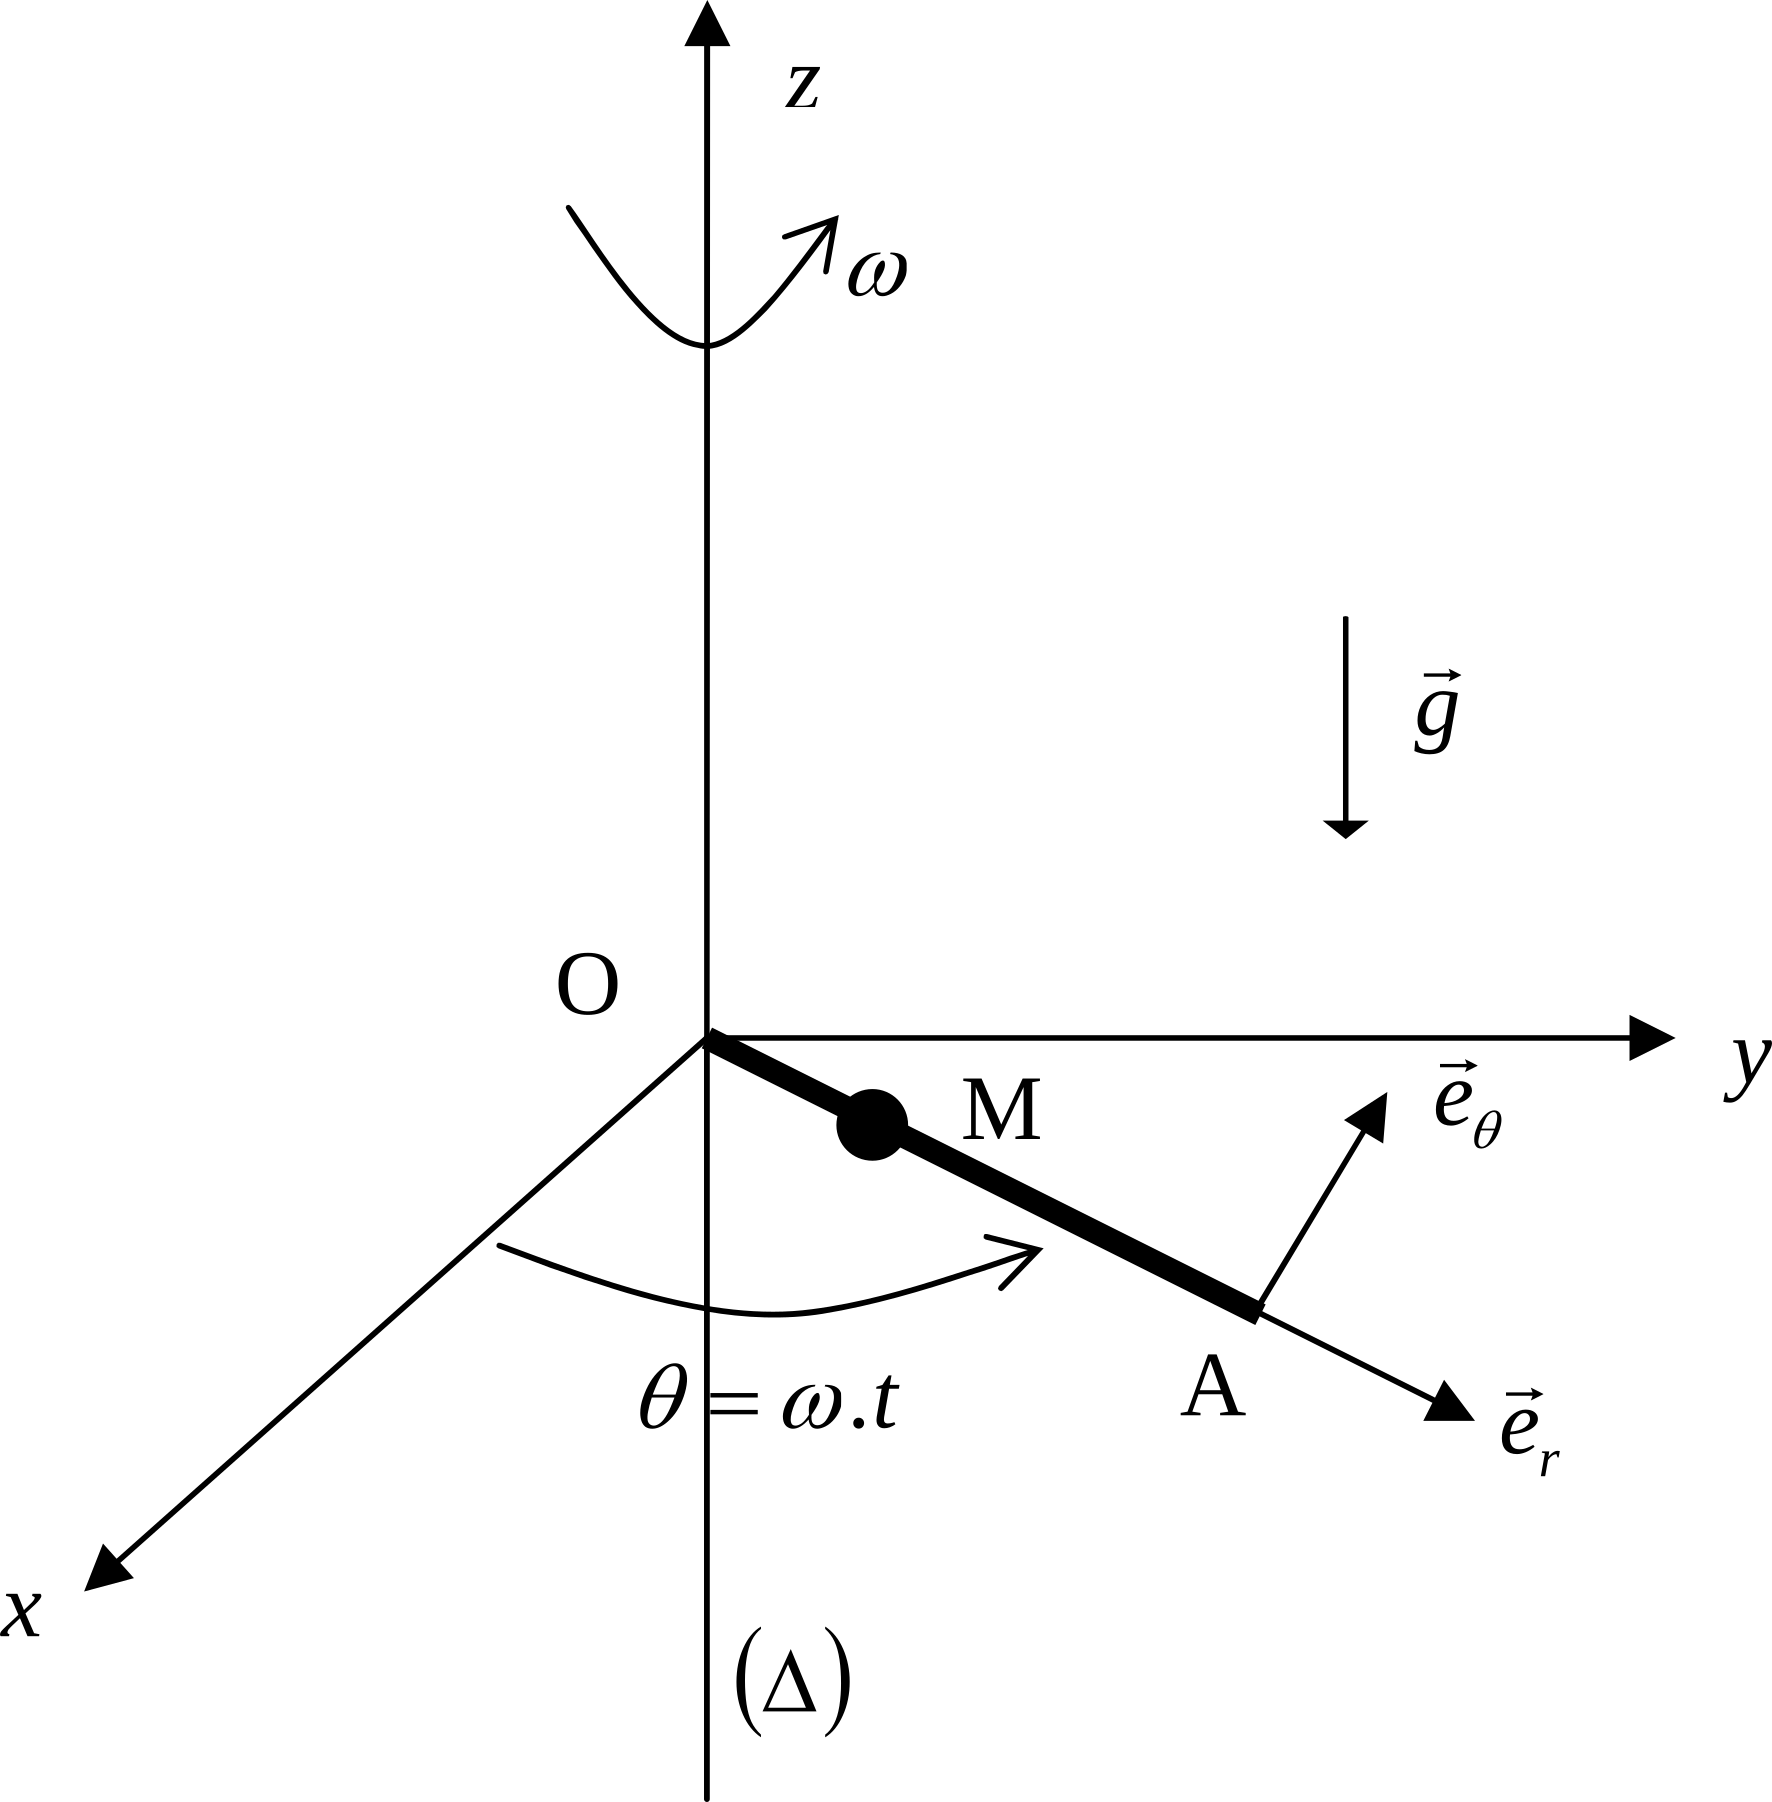
\includegraphics[width=\linewidth]{anneau_tige_rot-plain}
    \end{center}
\end{minipage}
L'anneau est libéré sans vitesse initiale par rapport à la tige, à une
distance $r_0$ du point O (avec $r_0 < \ell$). On repère la position de
l'anneau sur la tige par la distance $r = \OMr$ entre le point O et l'anneau
M.
\bigbreak
\begin{enumerate}
    \item Faire un bilan des forces agissant sur l'anneau en les projetant dans
        la base $(\er,\et,\ez)$. En appliquant le
        principe fondamental de la dynamique, établir l'équation différentielle
        vérifiée par $r(t)$.
    \item Intégrer cette équation différentielle en prenant en compte les
        conditions initiales définies précédemment, et déterminer la solution
        $r(t)$ en fonction de $r_0$, $\w$ et $t$.
    \item Exprimer les composantes de la réaction $\Rf$ de la tige sur M dans la
        base $(\er,\et,\ez)$ en fonction de $m$, $g$, $\rp$ et $\w$.
    \item Déduire de la question 2 le temps $\tau$ que va mettre l'anneau pour
        quitter la tige. On exprimera $\tau$ en fonction de $r_0$, $\ell$ et
        $\w$.
\end{enumerate}

\section{Pendule conique}

\hspace*{-0.75cm}
\begin{minipage}{0.70\linewidth}
    Dans un champ uniforme de pesanteur $\gf$ vertical et vers le bas, un point
    matériel M de masse $m$ tourne à la vitesse angulaire $\w$ constante autour de
    l'axe (O$z$) dirigé vers le haut en décrivant un cercle de centre O et de rayon
    $R$. M est suspendu à un fil inextensible de longueur $L$ et de masse
    négligeable, fixé en un point A de (O$z$). L'angle $\a$ de (O$z$) avec AM est
    constant. \bigbreak
    \begin{enumerate}
        \item Quel système de coordonnées utiliser~?
        \item Effectuer un bilan des forces s'appliquant à la masse et les écrire
            dans la base choisie.
        \item Appliquer le PFD puis exprimer $\cos\a$ en fonction de $g$, $L$ et
            $\w$. En déduire que la vitesse angulaire doit forcément être supérieure
            à une vitesse angulaire limite $\w_{\lim}$ pour qu'un tel mouvement
            puisse être possible.
        \item Que dire du cas où $\w$ devient très grande~?
        \item Application numérique~: calculer $\a$ pour $L = \SI{20}{cm}$ et $\w =
            \SI{3}{tours.s^{-1}}$.
    \end{enumerate}
\end{minipage}
\hfill
\begin{minipage}{0.25\linewidth}
    \begin{center}
        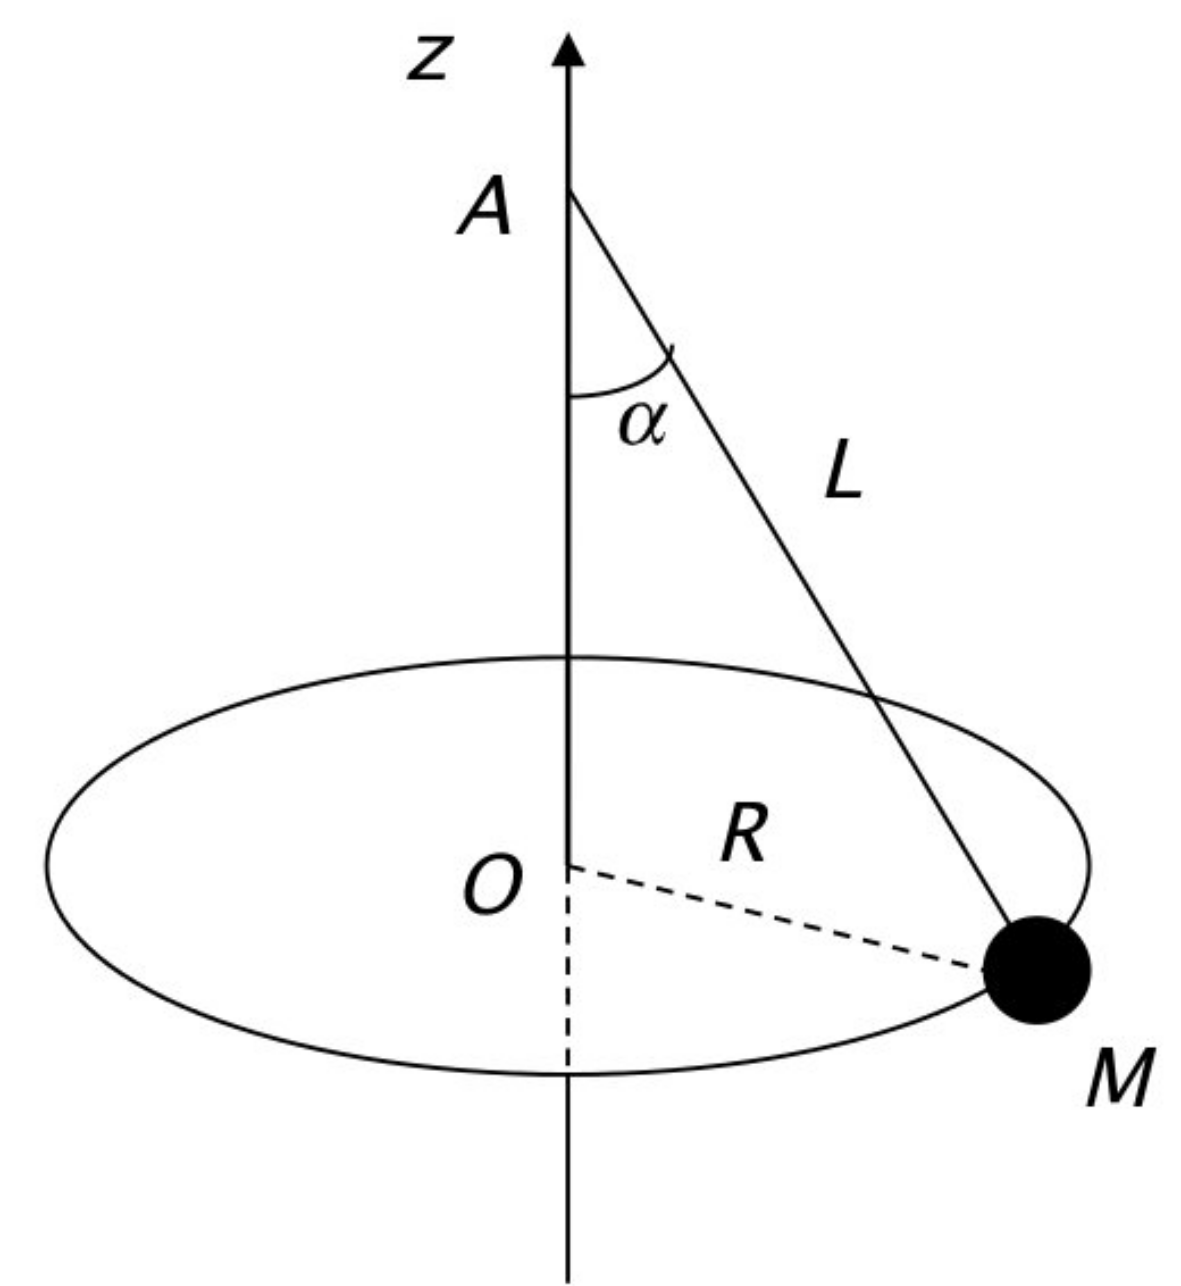
\includegraphics[width=\linewidth]{pendule_conique-plain}
    \end{center}
\end{minipage}

\end{document}
